\documentclass{article}
\usepackage{tikz}
\usepackage{amsmath} % Etiqueta split, text
\usepackage{amssymb} % Etiqueta mathbb
\usepackage{float}

\begin{document}
	
	% Ec.1.12
	\begin{equation}
		\begin{split}
			x'_{1} &= \sin \theta a_{11}x_{1} + a_{12}x_{2} \\
			x'_{2} &= a_{21}x_{1} + a_{22}x_{2}
		\end{split}	
		\label{ec1}	
	\end{equation}
	
	% Ec. 1.13
	\begin{equation}
		\begin{split}
			a_{12} &= \cos (x'_{1},  x_{2}) = \sin (\varphi), \\
			a_{21} &= \cos (x'_{2},  x_{1}) = \cos \left(\varphi+ \frac{\pi}{2} \right) = -\sin (\varphi)
		\end{split}
		\label{ec2}
	\end{equation}
	
	% Ec. 1.14
	\begin{equation}
		x'_{i} = \sum_{j = 1}^{2} a_{ij}x_{j},  \hspace{1cm} i = 1, 2
		\label{ec3}
	\end{equation}
	
	% Ec. 1.15
	\begin{equation}
		V'_{i} = \sum_{j = 1}^{N} a_{ij}V_{j}, \hspace{1cm} i = 1, 2, ..., N
		\label{ec4}
	\end{equation}
	
	% Ec. 1.16a
	\begin{equation}
		a_{ij} = \frac{\partial x'_{i}}{\partial x_{j}}
		\label{ec5}
	\end{equation}

	% Sin numero
	\begin{equation*}
		\begin{split}
			x\rightarrow x_{1} \\
			y\rightarrow x_{2} 			
		\end{split}
		\label{ec6}
	\end{equation*}
	
	% Sin número
	\begin{equation}
		\begin{split}
			a_{11} &= \cos \varphi  \hspace{1cm}  a_{12} = \sin \varphi \\
			a_{21} &= -\sin \varphi  \hspace{1cm} a_{22} = \cos \varphi
		\end{split}
		\label{ec7}
	\end{equation}
	
	%Ecuacion 1.22%
	\begin{equation}
		A_x = A cos \alpha \equiv A \cdot \hat{x}, \hspace{1cm} A_y = 
		A cos \beta \equiv A \cdot \hat{y}, \hspace{1cm} A_z = 
		A cos \gamma \equiv A \cdot \hat{z}.
		\label{ec8}
	\end{equation}
	
	%Ecuacion 1.23a%
	\begin{equation}
		\mathbf{A} \cdot (\mathbf{B} + \mathbf{C}) = 
		\mathbf{A} \cdot \mathbf{B}  + \mathbf{A}  \cdot \mathbf{C}
		\label{ec9}
	\end{equation}

	%Ecuacion 1.23b%
	\begin{equation}
		\mathbf{A}    \cdot (y\mathbf{B}) = 
		(y\mathbf{A}) \cdot \mathbf{B} =
		 y\mathbf{A}  \cdot \mathbf{B}
		\label{ec10}
	\end{equation}

	%Ecuacion 1.5%
	\begin{equation}
		\mathbf{B} = B_x\hat{x} +  B_y\hat{y} + B_z\hat{z}
		\label{ec11}
	\end{equation}

	%Sin nombre
	\begin{equation}
		(\varphi \rightarrow -\varphi)
		\label{ec12_1}
	\end{equation}

	%Ecuacion 1.16b%
	\begin{equation}
		x_j = \sum_{i=1}^{2} a_{i,j} x'_i 
		\hspace{1cm} \text{o} \hspace{1cm} 
		\frac{\partial x_j}{\partial x'_i} = a_{i,j}.
		\label{ec12}
	\end{equation}

	%Ecuación 1.17%
	\begin{equation}
		V'_i = 
		\sum_{j=1}^{N} \frac{\partial x'_i}{\partial x_j} V_j = 
		\sum_{j=1}^{N} \frac{\partial x_j}{\partial x'_i} V_j
		\label{ec13}
	\end{equation}

	%Ecuación 1.18%
	\begin{equation}
		\sum_{i} a_{i,j} a_{i,k} = \delta_{j,k}
		\label{ec14}
	\end{equation}

	%Ecuación 1.19%
	\begin{equation}
		\sum_{i} a_{j,i} a_{k,i} = \delta_{j,k}
		\label{ec15}
	\end{equation}

	%Ecuación 1.20%
	\begin{equation}
		\begin{split}
			\delta_{j,k} = 1 \hspace{1cm} &\text{para} \hspace{1cm}  j = k, \\
			\delta_{j,k} = 0 \hspace{1cm} &\text{para} \hspace{1cm}  j \neq k
		\end{split}
		\label{ec16}
	\end{equation}
	
	%Sin nombre
	\begin{equation}
		sin^2 \varphi + cos^2 \varphi = 1
		\label{ec17_1}
	\end{equation}
	
	%Ecuación 1.21%
	\begin{equation}
		\sum_{i} \frac{\partial x_j}{\partial x'_i} \frac{\partial x_k}{\partial x'_i} = 
		\sum_{i} \frac{\partial x_j}{\partial x'_i} \frac{\partial x'_i}{\partial x_k} = 
		\frac{\partial x_j}{\partial x_k}.
		\label{ec17}
	\end{equation}
	
	\begin{equation}
		\sum_{k} A'_k B'_k =
		\sum_{i} A_i  B_i
		\label{ec18}
	\end{equation}

	\begin{equation}
		\begin{split}
			\textbf{C} \cdot \textbf{C} 
			&= (\textbf{A} + \textbf{B}) \cdot (\textbf{A} + \textbf{B}) \\
			&= \textbf{A} \cdot \textbf{A} + \textbf{B} \cdot \textbf{B} + 2\textbf{A} \cdot \textbf{B}
		\end{split}
		\label{ec19}
	\end{equation}

	\begin{equation}
		\textbf{C} \cdot \textbf{C} = C^2
		\label{ec20}
	\end{equation}
	
	\begin{equation}
		\textbf{A} \cdot \textbf{B} = 
		\frac{1}{2} (C^2 - A^2 - B^2)
		\label{ec21}
	\end{equation}
	
	\begin{equation}
		C^2 = A^2 + B^2 + 2ABcos\theta
		\label{ec22}
	\end{equation}
	
	\begin{equation}
		\begin{split}
			A'_x B'_x + A'_y B'_y + A'_z B'_z =
			& \sum_{i} a_{x,i} A_i \sum_{j} a_{x,j} B_j
			\sum_{i} a_{y,i} A_i \sum_{j} a_{y,j} B_j \\
			& \sum_{i} a_{z,i} A_i \sum_{j} a_{z,j} B_j
		\end{split}
		\label{ec23}
	\end{equation}

	\begin{equation}
		\sum_{k} A'_k B'_k =
		\sum_{l} \sum_{i} \sum_{j} a_{l,i} A_i a_{l,j} B_j
		\label{ec24}
	\end{equation}
	
	\begin{equation}
		\sum_{k} A'_k B'_k = 
		\sum_{i} \sum_{j} \sum_{l} (a_{l,i}, a_{l,j}) A_i B_j = 
		\sum_{i} \sum_{j} \delta_{i,j} A_i B_j = 
		\sum_{i} A_i B_i
		\label{ec25}
	\end{equation}

	\begin{equation}
		\textbf{A} \cdot (\textbf{B} + \textbf{C}) = 
		A B_A + A C_A =
		A (\textbf{B} + \textbf{C})_A
		\label{ec26}
	\end{equation}

	\begin{equation}
		\textbf{W} = \textbf{F} \times \textbf{S}
		\label{ec27}
	\end{equation}

	\begin{equation*}
		\textbf{A} = 6 \hat{x} + 4 \hat{y} + 3 \hat{z}
		\label{ec28_1}
	\end{equation*}

	\begin{equation*}
		\textbf{B} = 2 \hat{x} - 3 \hat{y} - 3 \hat{z}
		\label{ec28_2}
	\end{equation*}

	\begin{equation*}
		\textbf{A} \cdot \textbf{B} = (12 - 12 - 9) = -9
		\label{ec28}
	\end{equation*}

	\begin{equation}
		\begin{split}
			|\textbf{A}| &= (36 + 16 + 9)^\frac{1}{2} = 
			(61)^\frac{1}{2} = 7.81, \\
			|\textbf{B}| &= (4 + 9 + 9)^\frac{1}{2} = 
			(22)^\frac{1}{2} = 4.69
		\end{split}
		\label{ec29}
	\end{equation}

	\begin{equation}
		\textbf{r} = \hat{x} x + \hat{y} y
		\label{ec30_1}
	\end{equation}

	\begin{equation}
		\textbf{n} \cdot \textbf{r} = 0
		\label{ec30}
	\end{equation}

	\begin{equation}
		\textbf{e}_m \cdot \textbf{e}_n = \delta_{m,n}
		\label{ec31}
	\end{equation}

	
	
	\section{Figura 1.6 }
	%%%%% Rotation of cartesian coordinate axes %%%%%
	\begin{figure}[H]
		\begin{center}
			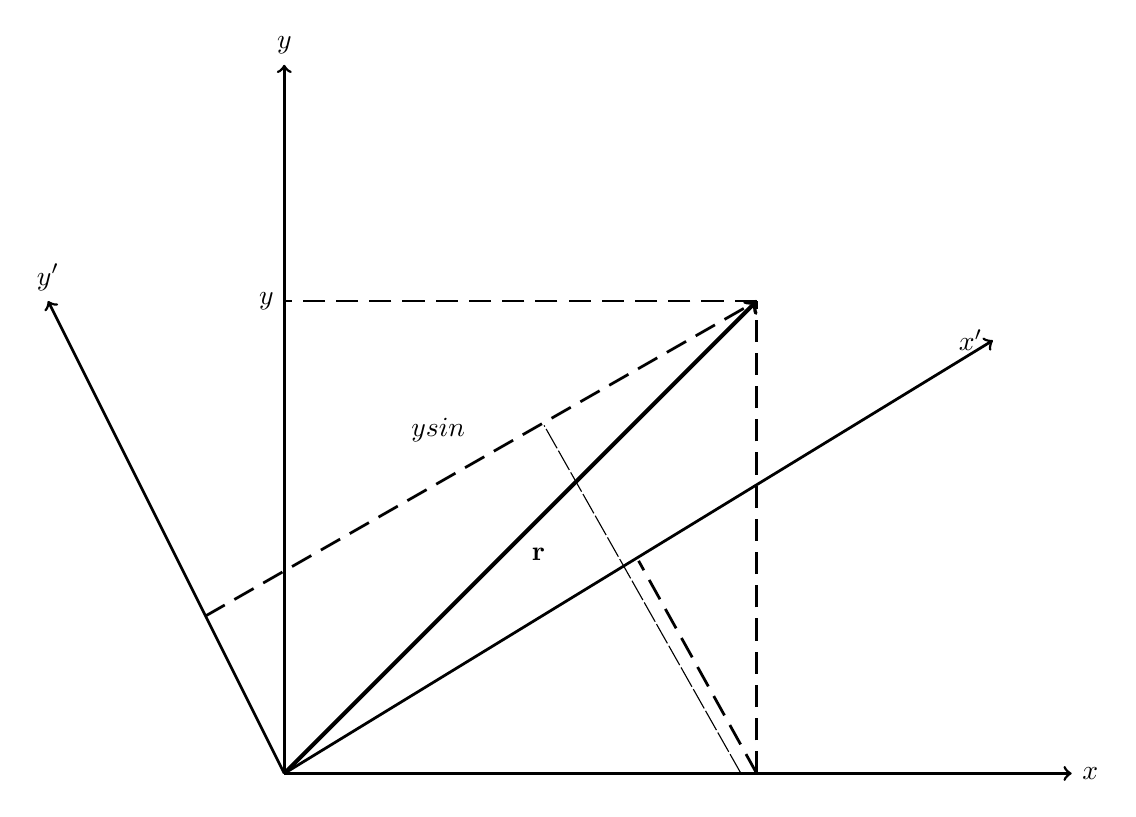
\begin{tikzpicture}
		%		\draw[lightgray] (0,0) grid (14,10);
				\draw[->, black, line width=1pt] (4,1)--(14,1) 
				node[right] {$x$}; % x
				\draw[->, black, line width=1pt] (4,1)--(4,10)
				node[above] {$y$}; % y
				\draw[->, black, line width=1.5pt] (4,1)--(10,7)
				node[midway, below right] {$\mathbf{r}$}; % r
				\draw[->, black, line width=1pt] (4,1)--(1,7)
				node[above] {$y'$}; % y'
				\draw[->, black, line width=1pt] (4,1)--(13,6.5)
				node[above, left] {$x'$};
				
				\draw[dash pattern=on 8pt off 4pt, black, line width=1pt] (10,7)--(4,7) node[left] {$y$};
				\draw[dash pattern=on 8pt off 4pt, black, line width=1pt] (3,3)--(10,7)
				node[midway, above left=2pt] {$y sin $};
				\draw[dash pattern=on 8pt off 4pt, black, line width=1pt] (10,1)--(10,7);
				\draw[dash pattern=on 8pt off 4pt, black, line width=1pt] (10,1)--(8.5,3.7);
				\draw[dash pattern=on 8pt off 1pt] (9.8,1)--(7.3,5.42);
				
			\end{tikzpicture}
		\end{center}
		\caption{.}
	\end{figure}

	
\end{document}
